\documentclass[10pt,twocolumn]{article}

\usepackage[utf8]{inputenc}
\usepackage[T1]{fontenc}
\usepackage{lmodern}
\usepackage[margin=1.9cm]{geometry}
\usepackage{amsmath,amssymb}
\usepackage{graphicx}
\usepackage{booktabs}
\usepackage{xcolor}
\usepackage{listings}
\usepackage{tikz}
\usetikzlibrary{positioning,fit,backgrounds,arrows.meta}
\usepackage[numbers,sort&compress]{natbib}
\usepackage[colorlinks=true,allcolors=blue!60!black]{hyperref}
\usepackage{authblk}
\usepackage{caption}
\captionsetup{font=small,labelfont=bf}

\definecolor{frozenblue}{HTML}{4C72B0}
\definecolor{jointred}{HTML}{C44E52}
\definecolor{accentgreen}{HTML}{55A868}
\definecolor{codebg}{HTML}{F5F5F5}

\lstset{
  basicstyle=\ttfamily\scriptsize,
  backgroundcolor=\color{codebg},
  keywordstyle=\color{frozenblue!80!black}\bfseries,
  commentstyle=\color{accentgreen!60!black}\itshape,
  stringstyle=\color{jointred},
  language=Python,
  breaklines=true,
  showstringspaces=false,
  columns=fullflexible,
  frame=single,
  framesep=3pt,
  rulecolor=\color{gray!40},
  aboveskip=6pt,belowskip=4pt,
}

\newcommand{\pp}{\,pp}

\title{\vspace{-1.2em}\textbf{DiffBio: End-to-End Differentiable Bioinformatics and the Case for\\ Jointly Optimized Preprocessing}}

\author[ ]{Mahdi Shafiei}
\affil[ ]{\small Avitai Bio \\ \texttt{mahdi@avitai.bio}}
\date{}

\begin{document}
\maketitle

\begin{abstract}
\noindent
Bioinformatics pipelines are built from discrete, non-differentiable stages, and the
choices that matter most---normalization, gene selection, and dimensionality
reduction---are frozen and tuned in isolation \emph{before} the downstream model ever
sees the data. We present \textbf{DiffBio}, a JAX/Flax library that reimplements core
bioinformatics operations as differentiable relaxations so that an entire analysis
workflow can be optimized end to end by gradient descent, and we use it to test a
concrete hypothesis: that jointly optimizing the dimensionality reduction with the task
model recovers task-relevant structure that a frozen, variance-maximizing projection
discards. On cell-type annotation over the Tabula Sapiens atlas, replacing frozen
principal component analysis (PCA) with a PCA-initialized learnable projection, trained
jointly with the classifier, improves held-out macro-F1 by
$\mathbf{+5.2\pp}$ at an aggressive reduction ($k{=}10$ components) on a
120{,}000-cell / 59-type subset, growing to $\mathbf{+10.2\pp}$ on a
193{,}000-cell / 87-type subset, with the largest gains ($+13.1\pp$) on rare cell types.
The advantage is regime-dependent: it is decisive under aggressive compression, survives
a stronger supervised gene-selection baseline ($+5.9\pp$), and narrows to a
non-significant $+1.6\pp$ when many components are retained ($k{=}50$)---joint
optimization helps precisely when one must compress hard, and is otherwise harmless.
Ablations attribute the gain to the learnable projection specifically, and a
differentiable ``soft-$k$'' operator recovers a good effective dimensionality without a
grid search. The effect then generalizes: across four further pipelines---DNA regulatory-
element classification, Perturb-seq perturbation identity, scATAC-seq annotation, and
variant calling---and two distinct reduction machineries (linear projection and
permutation-invariant read pooling), the same substitution yields $\mathbf{+7.5}$ to
$\mathbf{+16.9\pp}$ at aggressive reduction, while a no-bottleneck control on the same
variant data shows no gain, pinning the mechanism to compression that discards task signal.
DiffBio is open source.
\end{abstract}

\section{Introduction}

A modern single-cell or genomic analysis is a pipeline: raw measurements pass through
quality filtering, normalization, feature (gene) selection, dimensionality reduction, and
finally a task model such as a cell-type classifier or a variant caller. Each stage is
typically a \emph{discrete, hand-tuned} operation---a hard quality threshold, an
\texttt{argmax} base call, a fixed number of highly variable genes, a frozen
principal-component basis. Two consequences follow. First, discrete operations block
gradient flow, so the pipeline cannot be optimized as a whole. Second, and more
consequentially, the preprocessing is fit \emph{before}, and independently of, the
downstream objective: the projection that a variance-maximizing PCA chooses need not be
the projection that best serves cell-type annotation.

This staged, frozen design is near-universal in tools such as
Scanpy~\citep{wolf2018scanpy} and is effective, but it leaves a gap. In neighboring
fields, making the preprocessing \emph{learnable} and training it jointly with the task
has repeatedly paid off: learnable audio frontends outperform fixed mel-filterbanks
(LEAF~\citep{zeghidour2021leaf}, SincNet~\citep{ravanelli2018sincnet}), differentiable
preprocessing search beats fixed default pipelines on tabular data
(DiffPrep~\citep{li2023diffprep}), and learned augmentation policies beat hand-designed
ones~\citep{cubuk2019autoaugment}. In single-cell genomics, probabilistic models such as
scVI/scANVI~\citep{lopez2018scvi,xu2021scanvi} learn a latent representation jointly with
(optionally) the label, but within a single fixed generative model family rather than as
a general, composable, differentiable pipeline.

We bring the differentiable-preprocessing paradigm to bioinformatics. Our contributions
are:
\begin{enumerate}\itemsep2pt
\item \textbf{DiffBio}, an open-source JAX/Flax~\citep{jax2018,flax2020} library that
implements bioinformatics operators---alignment, variant calling, single-cell analysis,
epigenomics, RNA-seq, normalization, and more---as differentiable modules with a uniform
interface, so heterogeneous operators compose into pipelines that train end to end
(Section~\ref{sec:library}).
\item A \textbf{joint-optimization formulation} for the single-cell preprocessing-to-annotation
pipeline, in which a learnable, PCA-initialized projection is trained together with the
annotation model against the label loss, together with a differentiable
\emph{soft-$k$} operator that learns the effective number of components
(Section~\ref{sec:method}).
\item An empirical study establishing, with honest attention to where it does and does
\emph{not} hold, that joint optimization beats frozen PCA for cell-type annotation---by
$+5.2$ to $+10.2\pp$ macro-F1 under aggressive reduction, growing with atlas size and
concentrated on rare cell types, surviving a stronger supervised baseline, and narrowing
to insignificance when reduction is generous---and then \textbf{generalizing} it across
four further real-data pipelines and a second reduction machinery (permutation-invariant
read pooling), with a mechanistic no-bottleneck control that isolates the cause
(Section~\ref{sec:experiments}).
\end{enumerate}

\section{The DiffBio library}
\label{sec:library}

DiffBio provides differentiable implementations of core bioinformatics algorithms so that
heterogeneous analysis stages compose into a single pipeline trainable by gradient descent.
It is the biology-specific operator layer of a JAX/NNX scientific-ML stack
(Figure~\ref{fig:arch}), built on four foundation packages: \emph{Datarax} (operator and
dataflow contracts), \emph{Artifex} (reusable model-building and optimizer components),
\emph{Opifex} (advanced optimization primitives, including the GradNorm multi-loss balancer
used below), and \emph{Calibrax} (metrics and regression control), all atop Flax NNX and
JAX/XLA for GPU execution.

\subsection{Operator abstraction and dataflow}

Every operation is an \texttt{OperatorModule}: a Flax NNX module carrying a frozen-dataclass
configuration, validated at construction, and a single \texttt{apply} method that maps a
dictionary of named arrays to an updated dictionary (Listing~\ref{lst:operator}). Three
conventions make otherwise-incompatible operations interoperable and differentiable:
\begin{itemize}\itemsep1pt
\item \textbf{Dictionary dataflow.} Operators read the keys they need and forward the rest
untouched (e.g.\ \texttt{"counts"}$\to$\texttt{"features"}$\to$\texttt{"projection"}$\to$%
\texttt{"logits"}), so a normalizer, a projection, and a classifier chain without bespoke
glue.
\item \textbf{One-hot sequence encoding.} Sequences are $(\text{length}\times\text{alphabet})$
arrays rather than integer indices, so gradients flow through base identity---a prerequisite
for differentiating alignment and variant operators.
\item \textbf{Temperature-controlled smoothing.} Each discrete decision is a smooth
relaxation with a temperature that recovers the hard operation in the limit, giving training
an explicit bias/variance control.
\end{itemize}
Trainable state is declared as \texttt{nnx.Param} and fixed buffers (a frozen PCA anchor,
running statistics) as \texttt{nnx.Variable}. A single \texttt{nnx.split(model,\,nnx.Param)}
therefore exposes \emph{exactly} the trainable parameters to \texttt{jax.grad}, whether they
live in one operator or are scattered across a ten-stage pipeline---the mechanism that makes
end-to-end optimization automatic.

\begin{figure}[t]
\centering
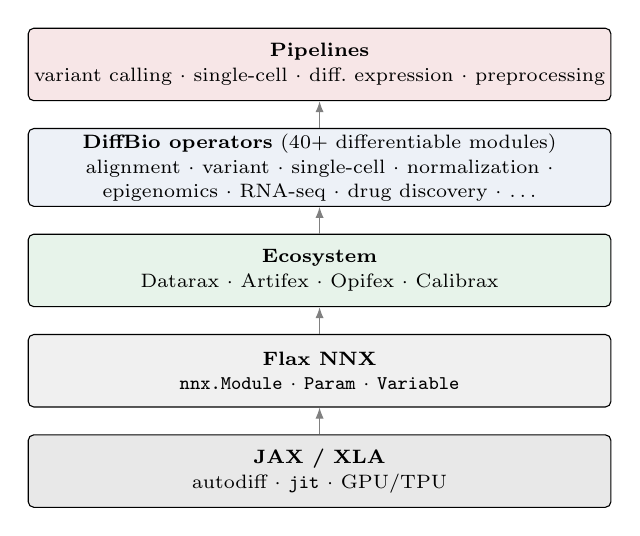
\begin{tikzpicture}[
  font=\scriptsize,
  layer/.style={draw,rounded corners=2pt,minimum width=7.4cm,minimum height=0.92cm,align=center,inner sep=2pt},
  node distance=0.34cm,
]
\node[layer,fill=jointred!14] (pipe)
  {\textbf{Pipelines}\\[1pt] \scriptsize variant calling \(\cdot\) single-cell \(\cdot\) diff.\ expression \(\cdot\) preprocessing};
\node[layer,fill=frozenblue!10,below=of pipe] (ops)
  {\textbf{DiffBio operators} (40+ differentiable modules)\\[1pt]
   \scriptsize alignment \(\cdot\) variant \(\cdot\) single-cell \(\cdot\) normalization \(\cdot\)\\[0.5pt]
   \scriptsize epigenomics \(\cdot\) RNA-seq \(\cdot\) drug discovery \(\cdot\) \(\dots\)};
\node[layer,fill=accentgreen!14,below=of ops] (eco)
  {\textbf{Ecosystem}\\[1pt] \scriptsize Datarax \(\cdot\) Artifex \(\cdot\) Opifex \(\cdot\) Calibrax};
\node[layer,fill=gray!12,below=of eco] (flax)
  {\textbf{Flax NNX}\\[1pt] \scriptsize \texttt{nnx.Module} \(\cdot\) \texttt{Param} \(\cdot\) \texttt{Variable}};
\node[layer,fill=gray!18,below=of flax] (jax)
  {\textbf{JAX / XLA}\\[1pt] \scriptsize autodiff \(\cdot\) \texttt{jit} \(\cdot\) GPU/TPU};
\draw[-{Latex[length=1.4mm]},gray] (jax) -- (flax);
\draw[-{Latex[length=1.4mm]},gray] (flax) -- (eco);
\draw[-{Latex[length=1.4mm]},gray] (eco) -- (ops);
\draw[-{Latex[length=1.4mm]},gray] (ops) -- (pipe);
\end{tikzpicture}
\caption{\textbf{DiffBio architecture.} A uniform \texttt{OperatorModule} interface lets
40+ differentiable operators across bioinformatics domains compose into end-to-end
pipelines, atop the Datarax/Artifex/Opifex/Calibrax ecosystem and JAX/Flax.}
\label{fig:arch}
\end{figure}

\subsection{Operator catalog}

DiffBio ships 40+ operators across the major bioinformatics domains
(Table~\ref{tab:catalog}): sequence alignment (a \texttt{logsumexp}-relaxed
Smith--Waterman~\citep{smith1981identification}, profile HMMs, soft multiple alignment),
variant calling (a differentiable pileup feeding a CNN caller, after
DeepVariant~\citep{poplin2018deepvariant}, plus copy-number segmentation and quality
recalibration), single-cell analysis, epigenomics, RNA-seq, statistical models, drug
discovery, genome assembly, and protein/RNA structure. The single-cell suite exercised in
this paper---learnable normalization, soft highly-variable-gene selection, differentiable
scaling and PCA, and the learnable-projection and soft-$k$ operators of
Section~\ref{sec:method}---is one column of this catalog; six end-to-end pipelines (variant
calling, enhanced variant calling, differential expression, single-cell, perturbation, and
preprocessing) are pre-assembled from it.

\begin{table}[t]
\centering\small
\caption{Representative DiffBio operator domains and the relaxation each relies on.}
\label{tab:catalog}
\begin{tabular}{@{}p{1.75cm}p{4.35cm}p{1.15cm}@{}}
\toprule
Domain & Representative operators & Relaxation \\
\midrule
Alignment & Smith--Waterman, profile HMM, soft MSA & log-sum-exp \\
Variant & pileup, CNN caller, CNV segmentation, quality recalibration & segment-sum \\
Single-cell & normalization, soft HVG, PCA, clustering, batch correction, RNA velocity & sigmoid, power \\
Normalization & VAE normalizer, UMAP, PHATE, learnable / orthonormal projection, matrix-free PCA, soft-$k$ & power, sigmoid \\
Epi./RNA-seq & peak calling, chromatin state, splicing PSI, motif discovery & sigmoid \\
Statistical & HMM, EM quantification, NB-GLM & log-sum-exp \\
Drug disc. & GNN message passing, fingerprints, AttentiveFP, ADMET & GNN \\
Structure & protein secondary structure, RNA folding & log-sum-exp \\
Multi-omics & Hi-C contact, spatial deconvolution/detection & segment-sum \\
\bottomrule
\end{tabular}
\end{table}

\subsection{Making discrete operations differentiable}

Four recurring relaxations replace the discrete primitives that block gradient flow, each
recovering its hard counterpart as the temperature $\to 0$: \emph{(i)~log-sum-exp} for
dynamic-programming maxima (alignment scores, HMM decoding); \emph{(ii)~sigmoid gates} for
hard thresholds (quality filtering, soft-$k$ component selection); \emph{(iii)~segment-sum}
for counting (pileup depth, feature aggregation), replacing a histogram with a weighted
accumulation; and \emph{(iv)~Markov-power accumulation} for diffusion operators (imputation,
pseudotime), replacing an eigendecomposition---whose gradient is unstable on the degenerate
spectra common in single-cell graphs---with repeated sparse matrix products.

\begin{lstlisting}[caption={The uniform operator interface: a learnable projection.},label={lst:operator},float=t]
class LearnableProjection(OperatorModule):
    def __init__(self, config, *, init_loadings, rngs):
        super().__init__(config, rngs=rngs)
        # fixed PCA anchor + zero-init learnable residual
        self.basis = nnx.Variable(init_loadings)   # frozen
        self.delta = nnx.Param(jnp.zeros_like(init_loadings))
        self.bias  = nnx.Param(jnp.zeros(config.n_components))

    def apply(self, data, state, metadata, *_):
        projection = self.basis[...] + self.delta[...]
        z = data["features"] @ projection + self.bias[...]
        return {**data, "projection": z}, state, metadata
\end{lstlisting}

\subsection{Composition and end-to-end training}

Operators compose through a \texttt{CompositeOperatorModule} with a sequential strategy,
with lightweight adapters renaming dictionary keys between stages; because composition
preserves each child's parameters, the assembled pipeline is one differentiable graph.
DiffBio's training utilities then optimize it end to end (Listing~\ref{lst:train}): an AdamW
optimizer from the Artifex factory over the \texttt{nnx.Param} leaves, deterministic
mini-batching, gradient clipping, and---when a preprocessing regularizer must be balanced
against the task loss---an Opifex GradNorm balancer that weights objectives by their
training rates rather than a hand-tuned coefficient. Calibrax supplies held-out metrics and
regression control.

\begin{lstlisting}[caption={Composing operators into a pipeline and training every stage's parameters end to end.},label={lst:train},float=t]
pipeline = CompositeOperatorModule(
  CompositeOperatorConfig(
    strategy=CompositionStrategy.SEQUENTIAL,
    operators=[LearnableNormalization(...), SoftHVG(...),
               DifferentiableScaler(...),
               LearnableProjection(..., init_loadings=V),
               LinearEmbeddingProbe(...)]),
  rngs=rngs)

# one optimizer trains every nnx.Param across all stages
opt = nnx.Optimizer(pipeline, create_optimizer(cfg), wrt=nnx.Param)
for batch in loader:
    grads = nnx.grad(loss_fn)(pipeline, batch)
    opt.update(pipeline, grads)
\end{lstlisting}

This paper validates the joint-optimization instantiation in depth on single-cell
annotation and then across four further pipelines (Section~\ref{sec:experiments}); broad
per-operator validation of the rest of the catalog is out of scope, and we keep the breadth
catalog (Table~\ref{tab:catalog}) deliberately separate from the rigorous case studies that
follow.

\section{Jointly optimized preprocessing}
\label{sec:method}

\paragraph{Setup.} Consider cell-type annotation. Let $X \in \mathbb{R}^{n \times g}$ be
raw counts for $n$ cells over $g$ genes. The standard frozen pipeline applies a fixed
transform $T$ (library-size normalization, $\log$, highly-variable-gene selection,
$z$-scoring) and a variance-maximizing projection $V \in \mathbb{R}^{h \times k}$ (the top
$k$ PCA loadings on the $h$ selected genes), then trains only a classifier $f_\phi$ on the
frozen features $Z = T(X)V$:
\begin{equation}
\min_{\phi}\; \mathcal{L}\big(f_\phi(T(X)\,V),\, y\big).
\end{equation}
$V$ is chosen to maximize retained \emph{variance}, which need not align with the
directions that separate cell types.

\paragraph{Joint objective.} We instead make the projection learnable, initialized at the
PCA solution, and train it jointly with the classifier:
\begin{equation}
\min_{\theta,\phi}\; \mathcal{L}\big(f_\phi(T(X)\,(V+\Delta_\theta)),\, y\big),
\end{equation}
where $\Delta_\theta$ is a residual initialized to zero, so training \emph{starts} exactly
at the frozen-PCA baseline and can only improve on the training objective before adapting
(the LEAF initialization recipe~\citep{zeghidour2021leaf}). Because $V$ is a fixed,
data-independent matrix, this objective is well defined under mini-batch stochastic
gradient descent, unlike re-estimating PCA per mini-batch (Section~\ref{sec:setup}).

\paragraph{Statistics are frozen, not re-estimated per batch.} $T$'s global statistics
(gene means/variances) and the PCA anchor $V$ are fit \emph{once} on the training split
and held as constants (\texttt{stop\_gradient}), following the batch-normalization
pattern~\citep{ioffe2015batchnorm} and DiffPrep's fit-once transform~\citep{li2023diffprep}.
This keeps the objective stationary and, critically, removes the activation-memory blowup
of backpropagating through the full-batch pipeline: only the projection and classifier are
on the gradient tape, so training an atlas-scale batch fits comfortably on a single GPU.

\paragraph{Learning the dimension.} The number of components $k$ is itself a design
choice. We additionally provide a differentiable \emph{soft-$k$} operator that keeps the
PCA directions fixed but learns a cumulative-variance coverage threshold, softly gating
the eigenvalue-ranked components; it recovers a hard truncation as its temperature
vanishes and, trained against the loss, selects an effective dimensionality without a grid
search.

\section{Experiments}
\label{sec:experiments}

\subsection{Setup}
\label{sec:setup}

\paragraph{Data.} We use the Tabula Sapiens human cell
atlas~\citep{tabulasapiens2022}: a 120{,}000-cell subset spanning six tissues with 59
cell types, and a broader 193{,}000-cell subset spanning all ten available tissues with 87
cell types. Cells are split 80/20 train/test, stratified by cell type; all preprocessing
statistics are fit on the training split only.

\paragraph{Arms.} Both arms share the frozen transform $T$ and differ only in the
reduction: (i) \textbf{Frozen PCA}---fixed top-$k$ loadings, only the classifier trains
(the standard pipeline); (ii) \textbf{Joint projection}---the PCA-initialized learnable
projection $V+\Delta_\theta$, trained jointly. Both feed an identical two-layer MLP
classifier and are trained by deterministic mini-batch AdamW (batch 4096, 100 epochs).
This isolates the effect of \emph{learning the reduction} from gene selection and
classifier capacity. We report held-out macro-F1 and balanced accuracy, mean $\pm$ s.d.
over three seeds, with a rare-cell-type breakdown (classes in the lowest quartile of
training frequency).

\paragraph{Baselines and scope.} Our controlled comparison is frozen PCA with an identical
classifier, which isolates the reduction. Comparison against jointly-trained generative
models (scVI/scANVI~\citep{lopez2018scvi,xu2021scanvi}) and other feature-selection
schemes is important and left to future work (Section~\ref{sec:limitations}); we also
compare against a stronger \emph{supervised} gene-selection baseline below.

\subsection{Joint optimization beats frozen PCA}

\begin{figure*}[t]
\centering
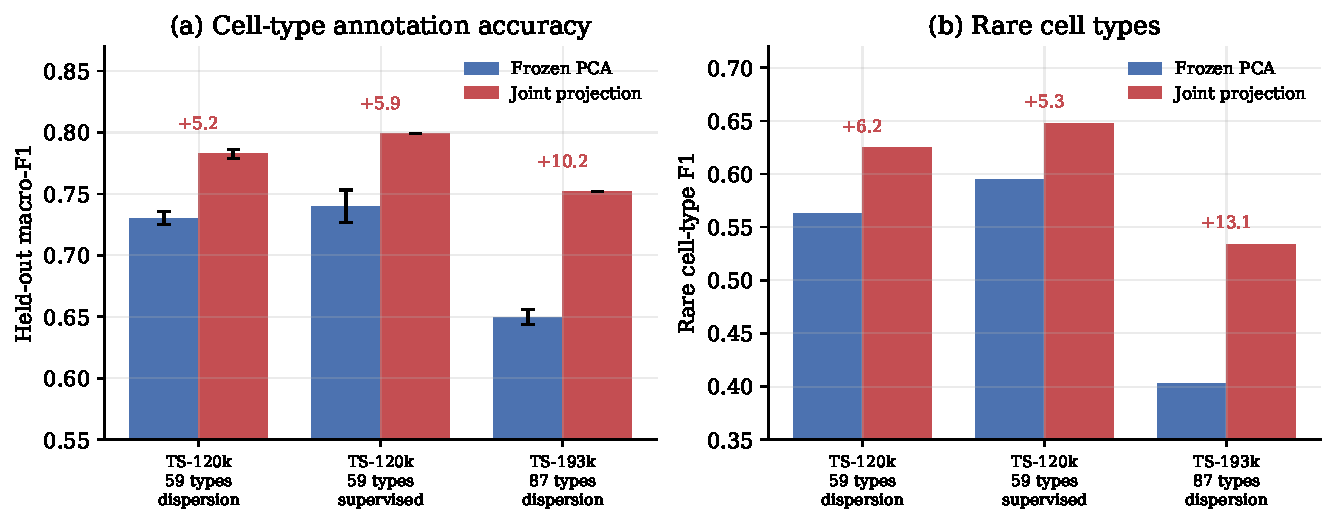
\includegraphics[width=0.86\textwidth]{figures/fig_main_result.pdf}
\caption{\textbf{Joint projection versus frozen PCA} at $k{=}10$ across atlases and
gene-selection methods (mean $\pm$ s.d., 3 seeds). \textbf{(a)} Overall held-out macro-F1;
annotations give the gain in percentage points. \textbf{(b)} F1 on rare cell types. The
joint projection wins in every condition, by more on the larger/harder 193k/87-type atlas,
and most on rare cell types.}
\label{fig:main}
\end{figure*}

At an aggressive reduction to $k{=}10$ components, the joint projection improves held-out
macro-F1 from $0.730{\pm}0.005$ to $0.783{\pm}0.003$ on the 120k/59-type atlas, a
$+5.2\pp$ gain with all three seeds positive; balanced accuracy rises correspondingly from
$0.706$ to $0.780$ (Table~\ref{tab:main}, Figure~\ref{fig:main}). On the larger and harder
193k/87-type atlas the absolute scores are lower (87 classes is a harder problem) but the
\emph{gain grows} to $+10.2\pp$ ($0.650 \!\to\! 0.752$). The effect is largest exactly
where annotation is hardest and most valuable: rare cell-type F1 improves by $+6.2\pp$ on
the 120k atlas and by $+13.1\pp$ ($0.403 \!\to\! 0.534$) on the 193k atlas.

\begin{table}[t]
\centering
\small
\caption{\textbf{Main result} at $k{=}10$ (held-out macro-F1, mean$\pm$s.d., 3 seeds).
``sup.''\ = supervised-Wilcoxon gene selection.}
\label{tab:main}
\begin{tabular}{@{}llccc@{}}
\toprule
Atlas & HVG & Frozen & Joint & Gain \\
\midrule
TS-120k/59 & disp. & $0.730{\pm}.005$ & $0.783{\pm}.003$ & $+5.2\pp$ \\
TS-120k/59 & sup.  & $0.740{\pm}.013$ & $0.799$          & $+5.9\pp$ \\
TS-193k/87 & disp. & $0.650{\pm}.006$ & $0.752$          & $+10.2\pp$ \\
\bottomrule
\end{tabular}
\end{table}

\paragraph{Not an artifact of weak gene selection.} A natural objection is that the frozen
baseline is handicapped by unsupervised (dispersion) gene selection. We therefore
strengthen it with \emph{supervised} highly-variable-gene selection---a one-vs-rest
Wilcoxon test that uses the training labels to pick the most class-discriminative
genes---for \emph{both} arms. The joint projection still wins, by $+5.9\pp$
(Table~\ref{tab:main}), marginally more than against dispersion selection. Learning the
projection directions helps orthogonally to how genes are selected.

\subsection{The gain is regime-dependent}

\begin{figure}[t]
\centering
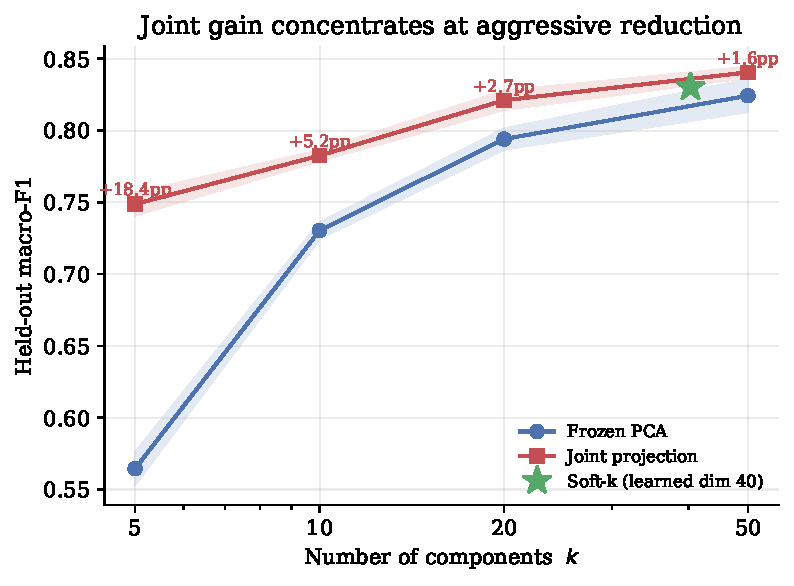
\includegraphics[width=0.94\columnwidth]{figures/fig_gain_vs_k.pdf}
\caption{\textbf{The joint gain concentrates at aggressive reduction.} Held-out macro-F1
of frozen PCA and the joint projection as a function of the number of components $k$
(TS-120k, mean $\pm$ s.d.). The advantage is large at small $k$ and narrows as $k$ grows
and the frozen basis already retains near-sufficient signal. The differentiable soft-$k$
operator ($\star$) learns an effective dimensionality of $\sim$40 and matches the best
fixed $k$ without a grid search.}
\label{fig:gainvk}
\end{figure}

Figure~\ref{fig:gainvk} is our central result. Sweeping the number of components, the joint
advantage is largest under aggressive compression and shrinks monotonically as $k$ grows:
from $+18.4\pp$ at $k{=}5$ (frozen $0.565{\pm}.011$, joint $0.749{\pm}.008$), through
$+5.2\pp$ at $k{=}10$ and $+2.7\pp$ at $k{=}20$, to only $+1.6\pp$ at $k{=}50$
(frozen $0.824{\pm}.011$, joint $0.841{\pm}.004$), whose spread includes zero (one of three
seeds marginally negative)---not significant. The mechanism is intuitive: at small $k$ the
projection must discard most of the signal, so \emph{which} directions it keeps matters and
coupling them to the task pays off; at large $k$ the variance-maximizing basis already
retains nearly all task-relevant structure, leaving little to gain. Joint optimization thus
\emph{helps when one must compress hard---the common regime for atlas-scale, memory-bound,
or interpretable low-dimensional embeddings---and is harmless otherwise.} The
differentiable soft-$k$ operator, given a pool of 50 components, learns to keep an effective
$\sim$40 and reaches $0.830$, matching the best grid value without a search.

\subsection{The effect generalizes across modalities and machineries}
\label{sec:crossmodality}

The single-cell result is one instance of a general phenomenon. Wherever a pipeline
compresses its data through a frozen, task-agnostic reduction before a model, the same
substitution---initialize a learnable reduction at the frozen one and train it jointly---
should recover discarded task signal, most at aggressive compression. We test this on four
further pipelines spanning distinct data modalities and two different reduction
\emph{machineries}, always with the identical two-arm protocol, real data, and held-out
evaluation (Table~\ref{tab:crossmod}, Figure~\ref{fig:crossmod}).

\begin{table*}[t]
\centering
\small
\caption{\textbf{The joint gain across pipelines} at aggressive reduction ($k{=}5$; held-out
macro-F1, mean over 3 seeds, 5 for the no-bottleneck control). Four modalities and two
reduction machineries; the final row is a no-reduction-bottleneck control on the \emph{same}
variant data.}
\label{tab:crossmod}
\begin{tabular}{@{}lllccc@{}}
\toprule
Pipeline & Modality & Machinery & Frozen macro-F1 & Joint macro-F1 & Gain \\
\midrule
scRNA annotation   & expression   & linear projection      & $0.565$ & $0.749$ & $+18.4\pp$ \\
DNA regulatory elements & DNA sequence & linear projection & $0.636$ & $0.711$ & $+7.5\pp$ \\
Perturb-seq identity & perturbation & linear projection    & $0.031$ & $0.113$ & $+8.3\pp$ \\
scATAC annotation  & chromatin    & linear projection (LSI)& $0.476$ & $0.598$ & $+12.2\pp$ \\
Variant calling    & aligned reads& read pooling (set)     & $0.714$ & $0.883$ & $+16.9\pp$ \\
\midrule
\emph{Variant calling (no bottleneck)} & aligned reads & pileup image + CNN & $0.877$ & $0.867$ & $-1.1\pp$ \\
\bottomrule
\end{tabular}
\end{table*}

\begin{figure}[t]
\centering
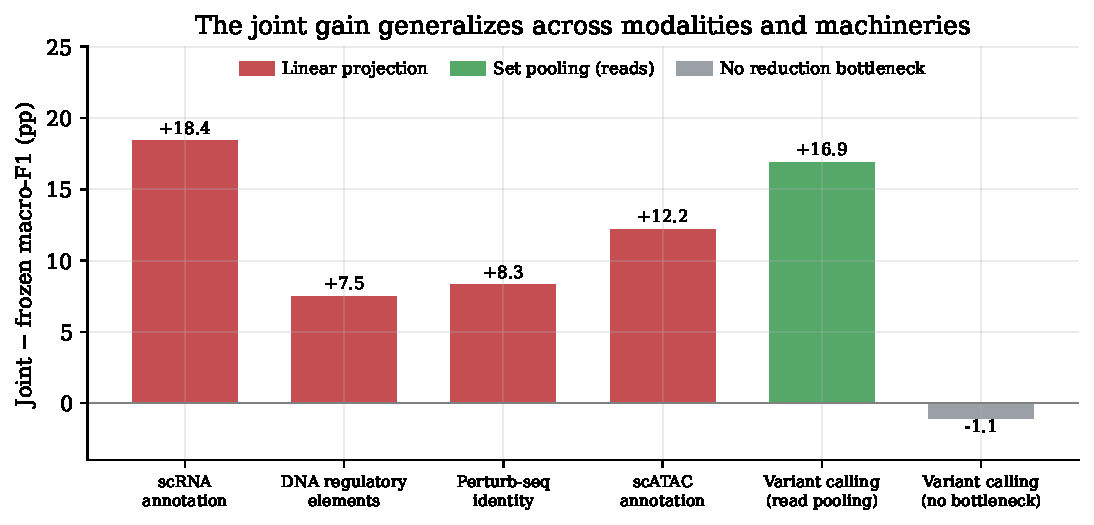
\includegraphics[width=0.99\columnwidth]{figures/fig_cross_modality.pdf}
\caption{\textbf{The joint gain generalizes.} Held-out macro-F1 improvement of the jointly
optimized reduction over the frozen one at aggressive compression ($k{=}5$), across five
pipelines and two machineries. The grey bar is the no-reduction-bottleneck control on
variant data, where the effect vanishes.}
\label{fig:crossmod}
\end{figure}

\paragraph{Four more modalities.} \emph{DNA regulatory elements:} classifying open-chromatin
regions from sequence (Genomic Benchmarks~\citep{gresova2023}, 174k sequences) with a frozen
$k$-mer-spectrum-plus-PCA frontend, the joint projection gains $+7.5\pp$ at $k{=}5$---and its
five learned dimensions exceed the standard 6-mer + linear-classifier baseline (logistic
regression $0.663$, linear SVM $0.697$; joint $0.711$).
\emph{Perturbation identity:} recovering which of 151 genetic perturbations a cell received
(a Perturb-seq atlas, target-gene-masked and split by experimental batch), a deliberately
hard 151-class task, it gains $+8.3\pp$ ($0.031\!\to\!0.113$ macro-F1, a $3.7\times$ relative
improvement). \emph{scATAC-seq annotation:} cell-type annotation of single-cell chromatin
accessibility (CATLAS~\citep{zhang2021catlas}, 154k cells, 36 types) with the standard
Signac TF-IDF plus latent-semantic-indexing (LSI) frontend~\citep{stuart2021signac}---a
genuinely different frozen reduction than PCA---it gains $+12.2\pp$. In all four the
gain-vs-$k$ signature recurs: large under aggressive compression, shrinking as $k$ grows.

\paragraph{scATAC in depth: a domain baseline and scaling.} As scATAC admits a
well-established annotation pipeline, we characterize it further. First, our frozen arm is
a faithful baseline, not a strawman: the standard Signac workflow---LSI at 50 components
followed by label transfer---reaches macro-F1 $0.790$ with logistic regression and $0.695$
with $k$-nearest-neighbors, bracketing our frozen MLP ($0.767$ at $k{=}50$), so the joint
gain is measured against competitive standard practice. Second, the gain scales with data
exactly as in single cells: sweeping the training-set size at $k{=}5$, the joint$-$frozen
gap runs $-7.1\pp$ (5k cells), $-2.7\pp$ (12k), $+4.3\pp$ (30k), $+7.5\pp$ (60k) to
$+12.2\pp$ (108k), crossing from negative to positive near $\sim$20k cells---a second,
independent crossover that replicates the single-cell one (Figure~\ref{fig:scaleabl}a).
Third, the gain is \emph{initialization-robust}: a \emph{randomly}-initialized learnable
projection reaches the same $0.60$ (vs.\ $0.59$ from the LSI init), so it is learning the
reduction, not inheriting the LSI subspace, and the uncompressed ceiling---all 12{,}000
TF-IDF features with no reduction---is $0.749$. Finally, the whole result \emph{replicates on
a disjoint set of 16 CATLAS donors} (127k cells, 41 types): $+8.1\pp$ at $k{=}5$ and
$+2.3\pp$ at $k{=}10$, the same signature on independent data.

\paragraph{A different machinery: pooling read evidence.} The pipelines above all learn a
linear projection. To test whether the effect is specific to that machinery we turn to
variant calling, where evidence is naturally reduced by pooling across sequencing reads.
From real GIAB HG002 chromosome-20 alignments~\citep{zook2019giab} we extract candidate
sites (true variants vs.\ sequencing-error look-alikes), featurize each read, reduce the
per-read features to $k$ dimensions and \emph{mean-pool over reads}---a permutation-invariant
set operation---before a classifier. Replacing the frozen per-read PCA with a jointly-trained
projection initialized from it improves macro-F1 by $+16.9\pp$ at $k{=}5$
($0.714\!\to\!0.883$), robustly across seeds. The variance-maximizing PCA never places the
low-variance but task-critical signal (a mismatch at the candidate position) in its top
components, so the frozen arm sits near $0.72$ across $k{=}3\!-\!20$ while the learnable arm
recovers it at once. The effect is not tied to linear-projection machinery.

\paragraph{A mechanistic null: no bottleneck, no gain.} The win requires a genuine lossy
reduction \emph{on the gradient path}, not merely a learnable hand-designed featurization.
On the same variant data we also made the DeepVariant-style pileup \emph{image} learnable---
its per-pixel channel encodings (base, quality, strand, mismatch) trainable and initialized
to reproduce the fixed encoding---feeding a convolutional classifier. Here nothing is
compressed: the network sees every read. Making the encoding learnable yields no improvement
($-1.1\pp$, within seed noise, with higher variance from the non-stationary frontend). Same
data and the same ``many learnable parameters plus a complex model,'' but no reduction
bottleneck, and the effect disappears---the control that pins the mechanism to compression.

\subsection{Attribution and scale}

\begin{figure*}[t]
\centering
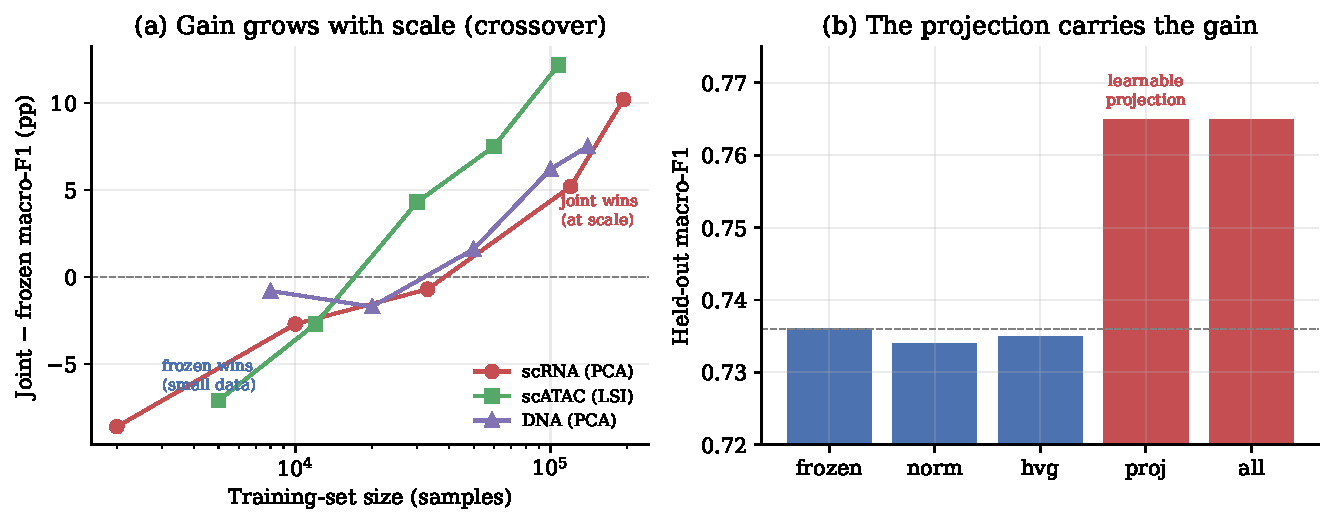
\includegraphics[width=0.86\textwidth]{figures/fig_scaling_ablation.pdf}
\caption{\textbf{(a)} The joint$-$frozen macro-F1 gap as a function of training-set size,
for three modalities: negative on small data, crossing zero near $\sim$20--40k samples and
rising to $+10.2\pp$ (scRNA), $+12.2\pp$ (scATAC), and $+7.5\pp$ (DNA) at scale---an
independent crossover in each. \textbf{(b)} Knob-attribution ablation (TS-120k, $k{=}10$):
making normalization or
gene-weighting learnable adds nothing over frozen; the learnable \emph{projection} carries
essentially the entire gain.}
\label{fig:scaleabl}
\end{figure*}

\paragraph{The projection carries the gain.} We ablate which learnable component is
responsible by training only one knob at a time (Figure~\ref{fig:scaleabl}b). Making
normalization or gene-weighting learnable leaves macro-F1 at the frozen baseline
($0.736 \!\to\! 0.734$/$0.735$); making the \emph{projection} learnable recovers the full
gain ($0.765$), and adding the other two on top does not improve further. The effect is
specifically about learning the reduction directions, consistent with the LEAF/DiffPrep
finding that the win lives in the learnable feature extractor. The attribution replicates on
the Perturb-seq task ($k{=}10$): the learnable projection recovers $+8.2$ of the $+8.3\pp$
total gain, while a learnable per-gene gate ($+2.7\pp$) and affine scaling ($+3.1\pp$)
contribute little on their own and do not stack.

\paragraph{The gain grows with scale.} Figure~\ref{fig:scaleabl}a plots the gap against
dataset size. On small data joint optimization \emph{hurts} (the frozen basis is a strong
low-variance regularizer): the gap is $-8.6\pp$ at 2{,}000 cells and remains negative
through $\sim$30k cells, crossing zero and turning decisively positive only at scale. The
scATAC and DNA pipelines show the same crossover independently (scATAC $-7.1\pp$ at 5k to
$+12.2\pp$ at 108k; DNA $-0.8\pp$ at 8k to $+7.5\pp$ at 140k), so this is not a single-dataset
artifact (Figure~\ref{fig:scaleabl}a).
This is the predicted win-condition---large data plus aggressive reduction---and it doubles
as an honest negative result (below).

\subsection{Trainable and orthonormal reduction bases}
\label{sec:trainablebasis}

The PCA-initialized residual projection is one point in a design space the operator library
now spans; two variants directly address the fixed PCA anchor it carries.
\emph{Trainable basis.} A matrix-free differentiable PCA---top-$k$ via randomized subspace
(power) iteration~\citep{halko2011randomized}, never forming the covariance---recomputes the
basis from the data each step, so gradients flow through the eigensolver to any upstream
learnable preprocessing: the basis \emph{itself} is trainable, with no fixed anchor. On the
DNA task ($k{=}5$), pairing it with a learnable per-feature scale lifts held-out macro-F1
from $0.632$ (frozen basis) to $0.669$ ($+3.7\pp$). \emph{Orthonormal basis.} A learnable
projection kept orthonormal by a QR retraction on the Stiefel manifold---no eigensolver, so
no eigengap instability---reaches $0.710$, matching the unconstrained learnable projection
($0.711$) at a third of its seed variance: on this task orthonormality is essentially free.
Both solvers stay finite where a differentiated dense eigendecomposition would
diverge~\citep{wang2019backprop}, realizing the trainable-basis extension at the cost of a
few matmuls and a QR.

\subsection{When joint optimization does not help}

Three regimes eliminate the advantage, and we report them plainly. \emph{Small data:} below
$\sim$30k cells the learnable projection overfits and underperforms frozen PCA
(Figure~\ref{fig:scaleabl}a); the frozen basis is a useful regularizer when labels are
scarce. \emph{Generous reduction:} at $k{=}50$ the gain is a non-significant $+1.6\pp$
(Figure~\ref{fig:gainvk}). \emph{No reduction bottleneck:} when the frozen stage merely
reformats the data rather than compressing it---the learnable-pileup-image control of
Section~\ref{sec:crossmodality}, where the model sees every read---making it learnable does
not help ($-1.1\pp$), even with many trainable parameters and a complex head. The method is
therefore not a universal replacement for frozen preprocessing but a targeted improvement
for the specific regime of large data reduced through an aggressive, lossy bottleneck.

\section{Discussion and limitations}
\label{sec:limitations}

Our study establishes the joint-optimization effect carefully but within a bounded scope,
and several limitations qualify it. \emph{(i) Atlas scope.} Both subsets derive from a
single atlas (Tabula Sapiens); although they span disjoint tissue sets and different
numbers of cell types, replication on an independent, differently-sequenced atlas (e.g.\
HLCA or a CELLxGENE census slice) is needed to rule out protocol-specific effects.
\emph{(ii) Baselines.} We isolate the reduction against frozen PCA; a full comparison
against jointly-trained generative models (scANVI) and other supervised feature-extraction
schemes remains future work. \emph{(iii) Depth vs.\ breadth of the cross-modality evidence.} The single-cell annotation
result is characterized in depth (atlas-size scaling, knob attribution, supervised-selection
control, soft-$k$); scATAC now adds a scaling curve, a domain-standard baseline,
initialization/no-reduction controls, and a disjoint-donor replication; DNA adds a scaling
curve and a domain baseline; and Perturb-seq adds the knob attribution
(Section~\ref{sec:crossmodality}). The main remaining gaps are the variant pipeline's own
depth---a comparison against a domain caller such as DeepVariant---and independent-dataset
replication of the DNA, Perturb-seq, and variant results.
\emph{(iv) Cost.} Joint training is more expensive than fitting frozen PCA once; freezing
the preprocessing statistics keeps the overhead modest (only the projection and classifier
are differentiated), but it is nonzero. \emph{(v) Uncertainty.} We report three seeds and
note per-seed signs; larger seed counts with paired significance tests would sharpen the
$k{=}50$ boundary.

\section{Future work}
\label{sec:future}

Several directions follow directly. \emph{Independent replication and scale:} extend the
mini-batch, fit-once design to 1M+ cell atlases (HLCA, CELLxGENE) via streaming covariance
estimation, testing whether the gain continues to grow. \emph{Stronger baselines:}
benchmark against scANVI and supervised metric-learning embeddings, and add a
random-projection and no-reduction control. \emph{Trainable-basis reductions:} the
matrix-free differentiable PCA and Stiefel orthonormal projection of
Section~\ref{sec:trainablebasis} are now in the library and validated on one task; scaling
them to the atlas-size joint-optimization experiments---replacing the fixed anchor entirely
while retaining stability~\citep{wang2019backprop}---is the natural next step.
\emph{Deepen the cross-modality results:} with scATAC now characterized in depth (scaling,
domain baseline, controls, disjoint-donor replication), the priorities are the variant
pipeline's own depth---a domain-caller comparison such as DeepVariant---independent-dataset
replication of the DNA, Perturb-seq, and variant results, and further reduction machineries
(soft alignment, hidden-Markov decoding). \emph{Automated pipeline
search:} lift the fixed operator ordering into a differentiable pipeline search in the
spirit of DiffPrep~\citep{li2023diffprep}, using DiffBio's uniform operator interface.

\section{Availability and reproducibility}

DiffBio is open source (MIT license) and built on JAX~\citep{jax2018} and Flax
NNX~\citep{flax2020}. All operators, the joint-training utilities, and the benchmark
harness used here ship with the library, with unit tests and fixed random seeds; the
figures in this paper are regenerated from the recorded benchmark outputs by a single
script. Preprocessing statistics are fit on training splits only, and every reported
number is a mean over at least three seeds.

{\small
\bibliographystyle{unsrtnat}
\bibliography{references}
}

\end{document}
